\newpage
\subsection{Progettazione di dettaglio e codifica}
Questo periodo inizia il giorno dopo la \textit{Revisione di Progettazione}(16/03/2019) e si conclude
con la consegna dei documenti per la \textit{Revisione di Qualifica}(12/04/2019). Le attività principali sono:
\begin{itemize}
	\item{\textbf{Incremento e Verifica:} all’inizio del periodo vengono svolte attività di Incremento e Verifica su vari documenti;}
	\item{\textbf{Glossario:} questa attività comprende sia il miglioramento del Glossario che l’aggiunta di nuovi termini;}
	\item{\textbf{Codifica:} questa attività consiste nella scrittura del codice e nella sua verifica secondo quanto indicato nella \textit{Definizione di Prodotto};}
	\item{\textbf{Lettera di presentazione:} questa attività prevede la stesura della lettera di presentazione per la \textit{Revisione di Qualifica}.}
\end{itemize}

\begin{figure}[h!]
	\centering
	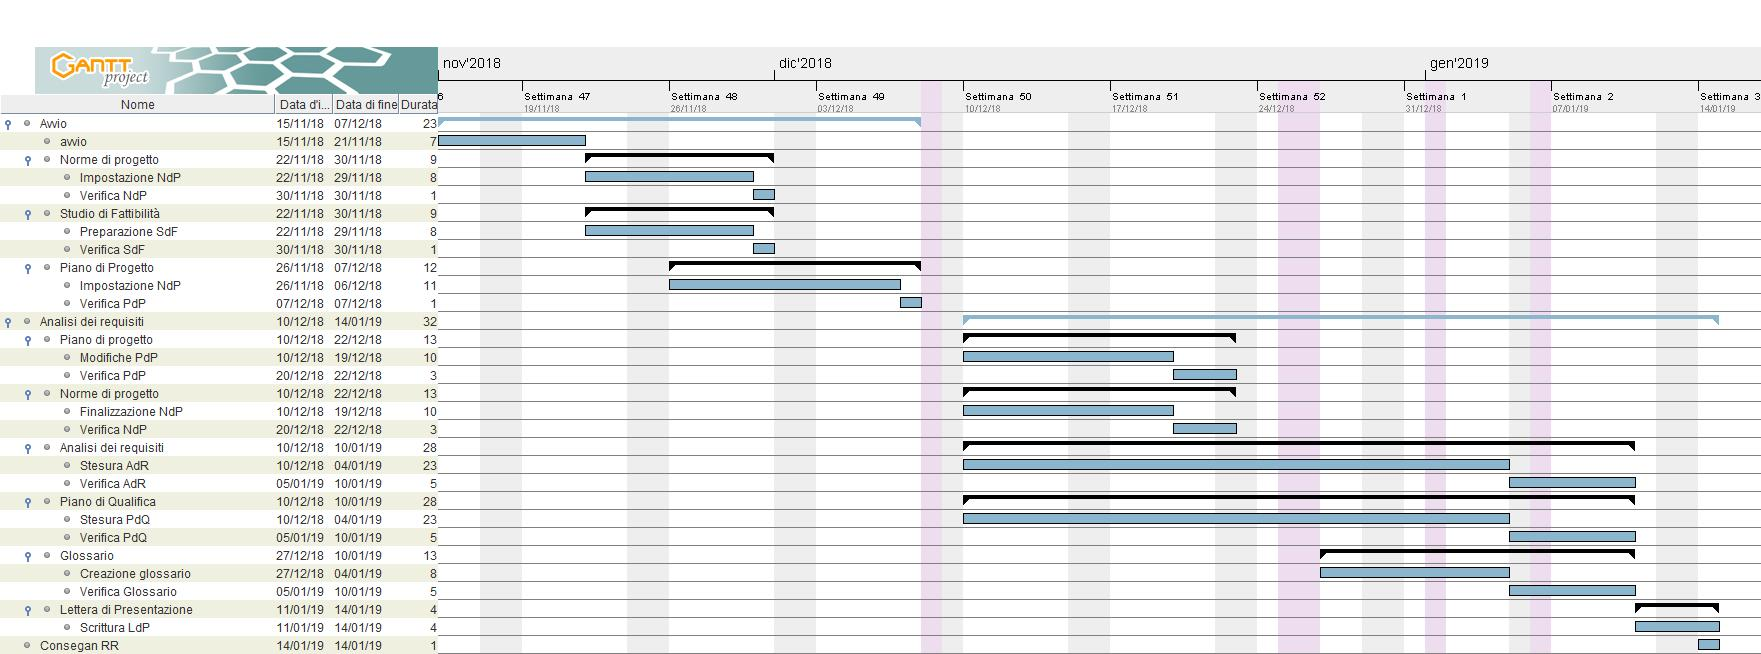
\includegraphics[width=\textwidth]{Gantt_terza_fase.jpg}
	\caption{Diagramma di Gantt del periodo di Progettazione di dettaglio e codifica}
\end{figure}

\begin{figure}[h!]
	\centering
	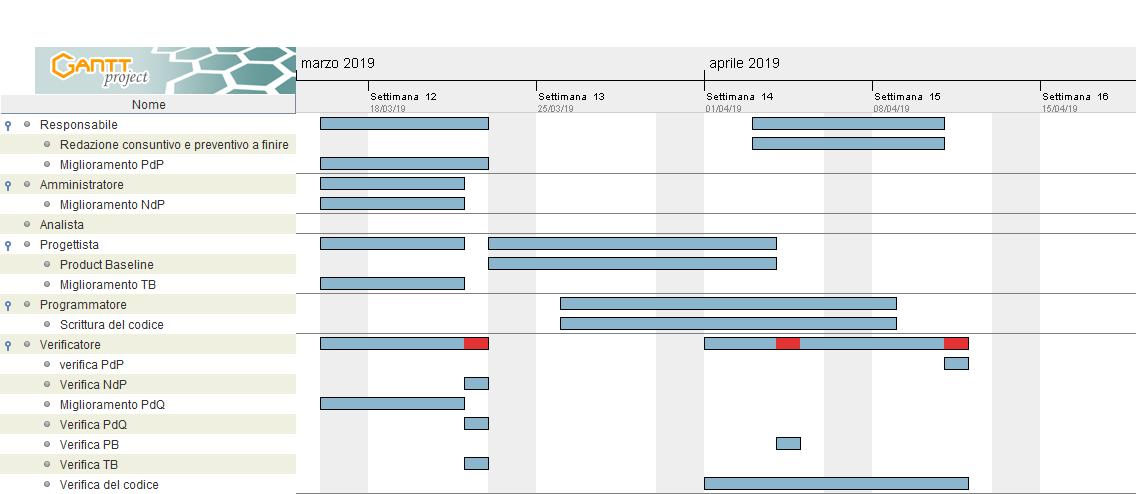
\includegraphics[width=\textwidth]{Gantt_terza_fase_risorse.jpg}
	\caption{Diagramma di Gantt delle risorse del periodo di Progettazione di dettaglio e codifica}
\end{figure}

\begin{table}[h!]
	\centering
	\renewcommand{\arraystretch}{2} 
	\rowcolors{2}{gray!25}{white}
	\begin{tabular}{|l|p{5cm}|p{5cm}|}
		\rowcolor{orange!50}
		\multicolumn{3}{|c|}{\textbf{Suddivisione temporale}}\\
		\hline
		\textbf{Ruolo} & \textbf{16/03/19 - 29/03/19} & \textbf{29/03/19 - 12/04/19} \\
		\hline
		\textbf{Responsabile} & \mat & \mar \\
		\hline
		\textbf{Amministratore} & \gia & \daG  \\
		\hline
		\textbf{Analista} & - & -  \\
		\hline
		\textbf{Progettista} & \parbox{5cm}{\pie \\ \mic} & \daL \\
		\hline
		\textbf{Programmatore} & \parbox{5cm}{\daG \\ \mar}& \parbox{5cm}{\mat \\ \mic \\ \pie}\\
		\hline
		\textbf{Verificatore} & \daL & \gia \\
		\hline
	\end{tabular}
	\caption{Suddivisione temporale del periodo di Progettazione di dettaglio e codifica}
\end{table}
